\chapter{Marco Teórico}%\phantom{\cite{beetz09ijcss}}
%\textcolor{red}{En desarrollo!!!!}.

\section{GPU}
\subsection{Definición}

Las unidades de procesamiento gráfico se encargan de rápidamente renderizar (representar) objetos 3D en forma de píxeles en la pantalla de la computadora, típicamente, por medio de arquitecturas de hardware basadas en la técnica de rasterización.
A continuación se mencionan las etapas principales del pipeline de gráficos convencional [\cite{Akenine2008}]:
\begin{enumerate}

\item El programa de usuario proporciona los datos al GPU en la forma de primitivas como puntos, líneas y polígonos que describen la geometría 3D. 
\item Etapa geométrica: las primitivas geométricas son procesadas en base a los vértices y son transformados de coordenadas 3D a triángulos 2D en la pantalla.. 
\item Etapa de rasterización: en esta etapa se dibuja una imagen mediante el uso de los datos anteriormente generados así como de los cálculos computacionales por píxel. La salida es un conjunto de píxeles donde cada píxel posee sus propios atributos (color, sombras, etc).  

\end{enumerate}

Los conjuntos de datos muy grandes que deben ser visualizados en tres dimensiones normalmente son creados usando representaciones de superficies mediante el dibujo de primitivas geométricas que crean mallas poligonales (en la mayoría de casos son mallas triangulares), pero las técnicas convencionales al usarse en el renderizarizado de datos volumétricos producen pérdidas en la visualización. Las técnicas de  renderización de volumen tienen más información que los métodos de renderización por superficie pero poseen una mayor complejidad y mayores tiempos de renderización [\cite{Akenine2008}].


\section{Raycasting}

A continuación, se presentan detalles acerca del algoritmo de raycasting en el cual se basa el GPU Theia para su funcionamiento.

\subsection{Definición}

El algoritmo de raycasting funciona haciendo cálculos a un píxel a la vez, y para cada píxel la tarea básica es encontrar el objeto que es observado en la posición correspondiente a ese píxel en la imagen, o sea parte del observador hacia los objetos a visualizar contrario al método por rasterización. Se puede decir que cada píxel ve en una dirección distinta y cualquier objeto que es observado por un píxel debe intersectar el rayo proveniente desde el punto de vista de la cámara. El objeto esperado es aquel que es intersectado primero por el rayo más cercano a la cámara. Una vez que el objeto es encontrado, se emplea el punto de intersección, la superficie normal, y alguna otra información del objeto para definir el color de cada píxel [\cite{Shirley2009}]. 

Entonces se puede decir que un algoritmo de raycasting tiene tres partes básicas:

\begin{enumerate}

\item Generación de rayo: donde se calcula el origen y la dirección de cada rayo (vector) del píxel correspoendiente en la vista de la cámara.
\item Intersección de rayo: donde se determina el objeto más cercano en la intersección del rayo proveniente de la cámara.
\item Shading: donde se calcula el color del píxel basado en los resultados de la intersección de rayos.

\end{enumerate}

Con el objetivo de generar rayos, primero se necesita una representación matemática de un rayo. Un rayo en realidad es solo un punto de origen y una dirección propagación. El rayo consiste en una línea paramétrica en 3D que va desde el ojo llamado punto \textit{e}, hasta un segundo punto \textit{s} ubicado en el plano de la imagen. La ecuación del rayo viene dada por:: 

\begin{equation}
\label{eq:ray_definition}
  p(t) = e+t(s-e)
\end{equation}

Esta fórmula implica que se empieza en el punto e y se avanza a través del vector s-e hasta llegar al punto p. Valores negativos de t implican que se encuentra el rayo detrás del ojo.

Un seudocódigo sobre el algoritmo de raycasting se muestra se muestra abajo en el seudocódigo \ref{ray}.

\begin{algorithm}
\caption{Algoritmo de Raycasting}\label{ray}
\begin{algorithmic}[1]
\Procedure{Ray-cast}{}
\For{$\textit{ cada pixel}$}
\State $\textit{ Construya un rayo desde el ojo}$
\For{$\textit{ cada objeto en la escena}$}
\State $\textit{ Encuentre la intersección con el rayo}$
\State $\textit{ Guarde esta intersección si es la más cercana}$
\EndFor
\EndFor
\EndProcedure
\end{algorithmic}
\end{algorithm}


%\begin{enumerate}

%\item For every pixel \# para cada píxel 
%\item \hspace{5 mm} Construct a ray from the eye \hspace{3 mm} // construya un rayo
%\item \hspace{5 mm} For every object in the scene \hspace{3 mm} // para cada objeto en la escena
%\item \hspace{10 mm}	 Find intersection with the ray \hspace{3 mm} // encuentre la intersección 	
%\item \hspace{10 mm} Keep if closest 				\hspace{3 mm} // Guarde el más cercano

%\end{enumerate}

En términos generales se puede afirmar que la técnica de raycasting evalúa el color de cada pixel en la imagen al disparar un rayo a través de la escena desde la posición del observador. Si el rayo intersecta el volumen, el color del pixel es calculado muestreando los datos a lo largo del rayo en un número finito de posiciones en el volumen  y combinando cada resultado en uno solo. Este método tiene una limitación al ejecutarse en los CPUs: para vólumenes de datos grandes el tiempo de renderización para una sola imagen es muy alto para visualización en tiempo real [\cite{Marques2009}]. En general el algoritmo de ray-casting, se enfoca en las técnicas de mayas para representar superficies para representar objetos.


\section{Arquitecturas con unidades de generación de rayos}

Existen en la literatura pocas referencias a unidades de raycasting o de ray tracing (variante del algoritmo de ray casting que genera rayos secundarios por medio de la recursión en el punto de incidencia del rayo original) que mencionen explícitamente dentro de su arquitectura la implementación de unidades de generación de rayos, las principales referencias son dos proyectos de hardware provenientes de la Universidad de Saarland (SaarCOR y DRPU) y RayCore de la Universidad de Sejong (\cite{Nah2014}).  En los artículos no se mencionan detalles de cómo se implementaron unidades de generación de rayos, solo se hablan de ellas de forma muy general.

En el caso de la GPU de tipo raycasting Theia, las especificaciones arquitectónicas indican la necesidad de una Unidad de Generación de Rayos (RGU, por sus siglas en inglés). La RGU debe poseer un conjunto de instrucciones necesarias para el cálculo de la normalización de vectores tridimensionales empleados en las siguientes etapas de funcionamiento del GPU.

\subsection{SaarCOR}

SaarCOR es el nombre de la unidad de ray tracing que fue diseñado para un chip de uso específico que está conectado por medio de un sistema de bus "host" (huésped) a otros chips que están en la misma placa de computadora. SaarCOR está dividido en tres unidades principales: la unidad de generación de rayos y de "shading" (RGS), el núcleo de ray tracing (RTC) y una unidad de manejo de acceso a memoria (RTC-MI) [\cite{Schmittler2004}]. 

\subsection{DRPU}

DRPU es el diseño y la implementación de un ASIC para procesamiento de ray tracing que posee capacidades de programabilidad similares a un GPU convencional en la universidad de Saarland [\cite{Woop2006}]. La arquitectura consiste en dos partes principales: Unidades de Ray Casting (encargadas de las estructuras espaciales) y un Procesador de "Shading" (encargado de hacer labores de sombreado y de generación de rayos).  

\subsection{RayCore}

RayCore es el diseño y la implementación de una unidad de ray tracing para dispositivos móviles y de bajo consumo por parte de miembros de la Universidad de Sejong en Corea del Sur. Dentro de RayCore existen dos unidades principales: una Unidad de Creación de Árboles (TBU) y una Unidad de Ray-Tracing (RTU). Dentro de RTU hay una unidad de generación de rayos tanto primarios como secundarios definidos por la unidad Set-Up y por la unidad de "shading", respectivamente [\cite{Nah2014}].   

%\subsection{Vizard II}

\section{Arquitectura de TheiaV3}
\subsection{Introducción a TheiaV3}
TheiaV3 es la tercera iteración del GPU multinúcleo de tipo raycasting Theia. El proyecto Theia es un proyecto de la modalidad Open Source (Código Libre) para experimentar con el hardware gráfico 3D (\cite{Valverde}].

El principal objetivo del proyecto Theia es proveer un ambiente Open Source incluyendo un código RTL funcional, un ambiente de pruebas y un lenguaje libre de alto nivel y un compilador para programar a Theia. En el diseño de Theia se plantea, por asuntos de simplicidad de diseño, que utilice el formato de sus datos en punto fijo en vez de emplear punto flotante.

El hardware de Theia es descrito usando código RTL escrito en Verilog 2001. Para realizar una simulación completa del código RTL, se necesita tanto un conjunto de archivos que representan los parámetros de entrada, así como el código de usuario en representación binaria.  

\subsection{Descripción general del sistema}

Theia es una unidad de procesamiento gráfico (GPU) multinúcleo, que tiene distintos bloques que interactúan entre ellos con la finalidad de renderizar cuadros de imágenes.

En la figura se muestran los principales bloques funcionales de Theia así como la memoria principal que se encuentra en el exterior del GPU. La memoria principal es una memoria de tipo RAM que es empleada para almacenar las variables geométricas, el código, entre otros detalles.

\subsection{Unidad de Generación de Rayos}

La Unidad de Generación de Rayos (RGU por sus siglas en inglés) es un módulo de hardware encargado de la generación de las estructuras de datos que representan los rayos que son enviados a los otros módulos encargados de la intersección de los mismos. La RGU tiene un conjunto limitado de operaciones aritméticas así un conjunto de instrucciones propias orientadas a la generación de los rayos por lo que carece de instrucciones de control de flujo. En la figura \ref{fig:rgu} se puede ver los bloques principales del RGU donde los azules representan memorias y los verdes bloques de lógica, además a la par de cada flecha se encuentra el nombre que correspondería a ese flujo funcional.

\begin{figure}
	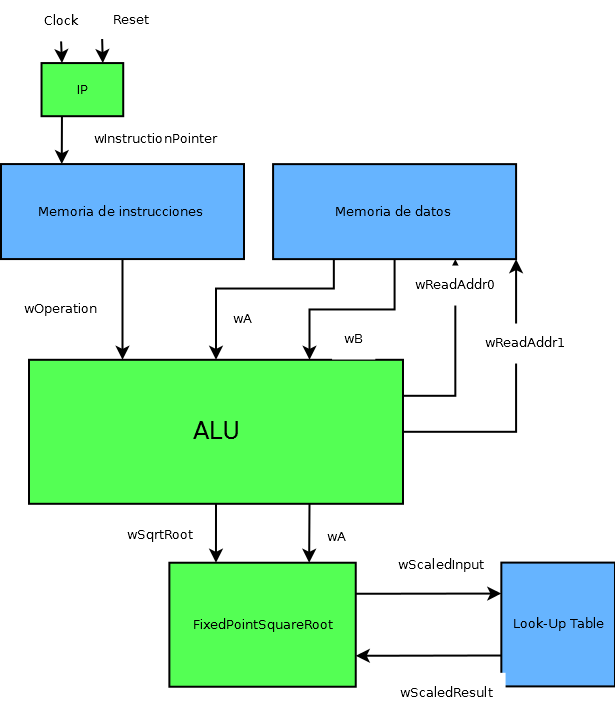
\includegraphics[width=1\linewidth]{images/rgu}
	\caption{Diagrama de los bloques funcionales del RGU} \label{fig:rgu}
\end{figure}

\section{Métodos de normalización}

La Unidad de Generación de Rayos de TheiaV3 debe realizar la operación del inverso de la raíz cuadrada con el objetivo de normalizar el rayo (vector) visto desde el observador, para lo cual se debe implementar dentro de
la unidad un mecanismo que permita calcular una aproximación por medio de instrucciones aritméticas simples y de una forma rápida.  A continuación se describen los métodos posibles. 

Existen varios tipos de posibles algoritmos para el cálculo de raíces cuadradas pero en realidad para la implementación en microprocesadores hay pocos, y estos caben en dos categorías: multiplicativos y sustractivos. Los métodos multiplicativos normalmente se implementan en hardware junto con el multiplicador de la unidad de punto flotante y permiten realizar operaciones rapidamente, y por otro los métodos sustractivos emplean hardware dedicado a estas operaciones, lo cual incrementa la latencia y los vuelve técnicas más lentas (\cite{Soderquist1997}].   

\subsection{Métodos multiplicativos}

Los algoritmos multiplicativos se suelen emplear para realizar cálculos estimados de raíces cuadradas usando iteraciones a partir de un estimado inicial. Emplear este tipo de técnicas reducen la ejecución de una operación de raíz cuadrada en una serie de multiplicaciones, sustracciones, y corrimientos de bits. Además vale la pena resaltar que estos métodos numéricos convergen cuadráticamente, lo cual implica que un estimado inicial apropiado preciso proporcionará resultados más precisos por cada iteración. Las técnicas empleadas frecuentemente en microprocesadores son los métodos de Newton-Raphson y de Goldschmidt, donde ambos métodos comparte muchos detalles en común pero se diferencian en el orden en que realizan las operaciones (\cite{Soderquist1997}].

\subsubsection{Newton-Raphson}

El método de Newton-Raphson es un método iterativo de convergencia cuadrática que emplea multiplicaciones sucesivas para aprovechar las capacidades de multiplicación rápida de los procesadores contemporáneos [\cite{Schulte1999}]. 

Al ser Newton-Raphson un método plenamente iterativo, con el objetivo de reducir las iteraciones que se realizan en los cálculos se suele emplear tablas de hardware las cuales se emplean como punto de partida en el proceso de iteraciones.

El método de Newton-Raphson se fundamenta encontrar la mejor aproximación posible al valor de las raíces o ceros de una función F(x) donde $F(x)=0$. 

Entonces mediante el método de Newton-Raphson si se inicia iterando a partir de un valor $X_0$ aproximado al valor deseado, entonces se tiene la expresión \ref{newton_raphson_definition}.


\begin{align} \label{newton_raphson_definition}
\begin{split}
  f'(x_0) &= \frac{f(x_0)}{x_0-x_1} 
\\
  x_1 &= x_0-\frac{f(x_0)}{f'(x_0)} 
\end{split}  
\end{align} 


Aplicando la definición del método de Newton-Raphson a la ecuación $x^{-2}-S=0$ donde la raíz es $\frac{1}{\sqrt{S}}$ se obtiene la expresión \eqref{eq:newton_raphson_square_root}:

\begin{equation}
\label{eq:newton_raphson_square_root}
  R_{i+1}=R_{i}(3-SR_{i}^{2})/2
\end{equation}

donde S es el valor de la base de la raíz y $R_{i}$ el valor del cálculo de la raíz cuadrada en la iteración i. El valor de la iteración 0 es el valor que debe salir de las tablas de aproximación.


\subsubsection{Goldschmidt}

El método de Goldschmidt para división y aplicada también para raíces cuadradas, surgió de la tesis de graduación de maestría de Ingeniería Eléctrica del MIT por parte de Robert Goldschmidt en 1964 [\cite{Goldschmidt1964}]. Esta técnica se basa en la aproximación de la raíz cuadrada por medio de productos sucesivos donde si $b_{0}$ es el valor de la base de la raíz cuadrada se busca que se cumpla que $b_{n}=b_{0}Y_{0}Y_{1}...Y_{n}=1$.

El método de Goldschmidt es ideal para aplicaciones que implementan de forma separada la multiplicación de la suma y en general se emplea en multiplicadores en pipeline. Un detalle de este método es que 

Las ecuaciones \eqref{eq:goldschmidt1} y \eqref{eq:goldschmidt2} son necesarias para el cumplimiento de este método numérico. El método de Goldschmidt, contrario al de Newton, no es autocorregible lo cual implica que existan errores acumulados [\cite{Markstein2004}].

\begin{equation}
\label{eq:goldschmidt1}
  b_{i}=b_{i-1}Y_{i-1}^{2}
\end{equation}

\begin{equation}
\label{eq:goldschmidt2}
  Y_{i}=(3-b_{i})/2
\end{equation}
  

%\subsection{SRT-Redundant}

%\subsection{Non-Restoring}

%\subsection{Wong-Goto}

\section{Punto fijo sin signo}

Una palabra de N-bits cuando es representada en la forma de un número racional en punto fijo, puede tomar los valores dados por el subconjunto P pertenecientes a los racionales no negativos como se observa en la ecuación \eqref{eq:subset}.

\begin{equation}
\label{eq:subset}
	P = \{p/2^{b}\quad |\quad 0 \leq p \leq 2^{N}-1, \quad p \in \mathbb{Z}\}
\end{equation}

En la ecuación anterior se tiene que P contiene $2^{N}$ elementos. Además la nomenclatura P(a,b) representa el subconjunto P, suponiendo que $a=N-b$.

Por otra parte, el valor de un número binario de N-bits X, perteneciente al subconjunto P está dado por la ecuación \eqref{eq:X}.
\begin{equation}
\label{eq:X}
   X = (1/2^{b}){\sum^{N-1}_{n=0}} 2^{n} x_{n}
\end{equation}

donde $X_n$ representa el bit n del número X. El rango de números que puede tomar como representación el número X es de 0 hasta $(2^{N}-1)/2^{b}=2^{a}-2^{-b}$.

La representación binaria de un número X en punto fijo de 6-bits donde la coma está ubicada a 2 bits a la derecha, o sea $b=2$, tiene la forma de $x_{3}x_{2}x_{1}x_{0}x_{-1}x_{-2}$. Por ejemplo en el diseño de Theia se emplea el punto fijo, el cual emplea la coma decimal en el bit 17 para la representanción de los números.

%\subsection{Reglas aritméticas}

%\begin{enumerate}

%\item \emph{Tamaño de las palabras:} El número bits requeridos para representar P(a,b) es a+b.

%\item \emph{Rango de palabras:} El rango de P(a,b) es $0 \leq X \leq 2^{a}-2^{-b}$.

%\item \emph{Multiplicación:} $P(a,b)*P(c,d)=P(a+c,b+d)$.

%\item \emph{División:} $P(a,b)/P(c,d)=P(a+c, \lceil log_{2}(2^{c+b}-2^{b-d}) \rceil)$. 

%\item \emph{Extraer los bits más significativos:} Si define la operación H(P(a,b)) como la extracción de la parte más significativa y a L(P(a,b)) como la operación para extraer la parte menos significativa, entonces se tiene que $H(P(a,b))=P(a, n-a)$ y $L(P(a,b))=P(n-b,b)$. 		

%\item \emph{Shift:} $P(a,b) \gg n = P(a-n,b+n)$. 	

%\end{enumerate}

\section{Verificación funcional}

\subsection{Generalidades}

Un ambiente de verificación funcional modela el universopara el diseño y debe soportar toda las acciones que pueden ocurrir sobre él. Este ambiente se conoce como banco de pruebas o “test bench” [\cite{Wile}].

Un ambiente básico de verificación consiste en las siguientes partes:

\begin{itemize}
\item Diseño bajo verificación (DUV).
\item Componente de estímulo.
\item Componente de monitoreo.
\item Componente de chequeo.
\item Scoreboard.
\end{itemize}

\subsection{Componente de estímulo}

Esta parte del banco de pruebas manipula las entradas del DUV (“driver”) e imita el comportamiento de entidades vecinas.
La generación de estímulos no deben restringirse
a lo que el DUV es capaz de recibir; de esta forma se estresa el DUV y se pueden encontrar condiciones límite que solo se pueden ver luego de millones de ciclos una prueba a nivel de sistema. Manipula las entradas del DUV (“driver”) [\cite{Wile}].

\subsection{Componente de chequeo}

La componente  de chequeo ("checker") es un tipo especial de monitor que solo colecta salidas del DUV encargado de validar que una funcionalidad del diseño se comporta de forma correcta [\cite{Wile}].
El checker necesita entender el estimulo para predecir el resultado funcional y comparar el resultado actual.
El checker tiene que revisar que se cumplan los siguientes puntos:
\begin{itemize}
\item Todas las respuestas sean recibidas.
\item Todas las salidas corresponden al valor esperado.
\item Que no haya actividad sin estimulo.
\end{itemize}

\subsection{Scoreboard}

Un scoreboard es una locación temporal que contiene información que el checker puede requerir.

Existen dos formas en que se puede establecer la relación entre el checker y el scoreboard:
\begin{itemize}
\item El checker contiene el modelo de referencia y el scoreboard se encarga de examinar las entradas para
almacenar la información necesaria cuando una transacción ocurre. El checker utiliza el modelo de referencia para transformar la información y comparar el resultados esperado con el resultado actual.
\item En el segundo método, el scoreboard tiene el modelo de referencia y calcula los valores esperados con base en los estímulos. Cuando el checker observa ciertos eventos en el DUV, llama al scoreboard para recibir el valor esperado y comparar.
\end{itemize}

\subsection{Tipos de checkers}

El trabajo de los “checkers” es asegurar que el DUV se comporta correctamente con base en el estimulo. Existen 4 fuentes principales de checkers:
\begin{enumerate}
\item Las entradas y salidas del diseño.
\item El contexto del diseño.
\item Las reglas de micro arquitectura del diseño.
\item La arquitectura del diseño.
\end{enumerate}


\subsubsection{Las entradas y salidas del diseño} 

Cualquier bug en el diseño en algún momento se debe manifestar a las salidas del diseño. El código de chequeo utiliza las entradas para predecir las salidas. Una inconsistencia ocurre cuando los datos provenientes del  Diseño bajo Verificación no coinciden con los datos de la componente chequeo. 

\subsubsection{El contexto del diseño} 

Cuando se verifica el Lenguaje de Descripción de Hardware (HDL) a bajo nivel es importante para el ingeniero verificador comprender el diseño entender la funcionalidad a alto nivel (por contexto). El ingeniero encargado de verificación debe conocer el proyecto a gran escala aún cuando solo deba encargarse de una específica sección del diseño.

\subsubsection{Las reglas de micro arquitectura del diseño} 

Los verificadores crean muchos de los checkers a partir de propiedades basadas en la microarquitectura o las estructuras internas del diseño, por lo que los ingenieros en verificación deben entender el interior del diseño.  

Se utiliza la especificación de la microarquitectura para definir propiedades como:
\begin{itemize}
\item Estados inválidos.
\item Transiciones invalidas.
\item Datos inválidos.
\item Temporización incorrecta de señales de control.
\item Tamaño de buffers y colas.
\end{itemize}

\subsubsection{La arquitectura del diseño} 
Mientras la microarquitectura define las estructuras que componen el diseño, la arquitectura dicta como debe actuar el diseño desde una especificación de alto nivel encargada protocols, unidades de procesamiento programable y estruturas del sistema en general.